\documentclass[tikz,border=8pt]{standalone}
\usepackage{amsmath}
\usepackage{xcolor}
\usetikzlibrary{positioning,arrows.meta,backgrounds,fit,calc,shapes.geometric}

\definecolor{cIn}{HTML}{ECEFF1}
\definecolor{cEnc}{HTML}{E3F2FD}
\definecolor{cBack}{HTML}{EDE7F6}
\definecolor{cStyle}{HTML}{FFE0B2}
\definecolor{cStyleE}{HTML}{E65100}
\definecolor{cFM}{HTML}{B2DFDB}
\definecolor{cFME}{HTML}{00695C}
\definecolor{cOut}{HTML}{F1F8E9}
\definecolor{cKnob}{HTML}{FFF176}
\definecolor{cTrain}{HTML}{FAFAFA}

\begin{document}
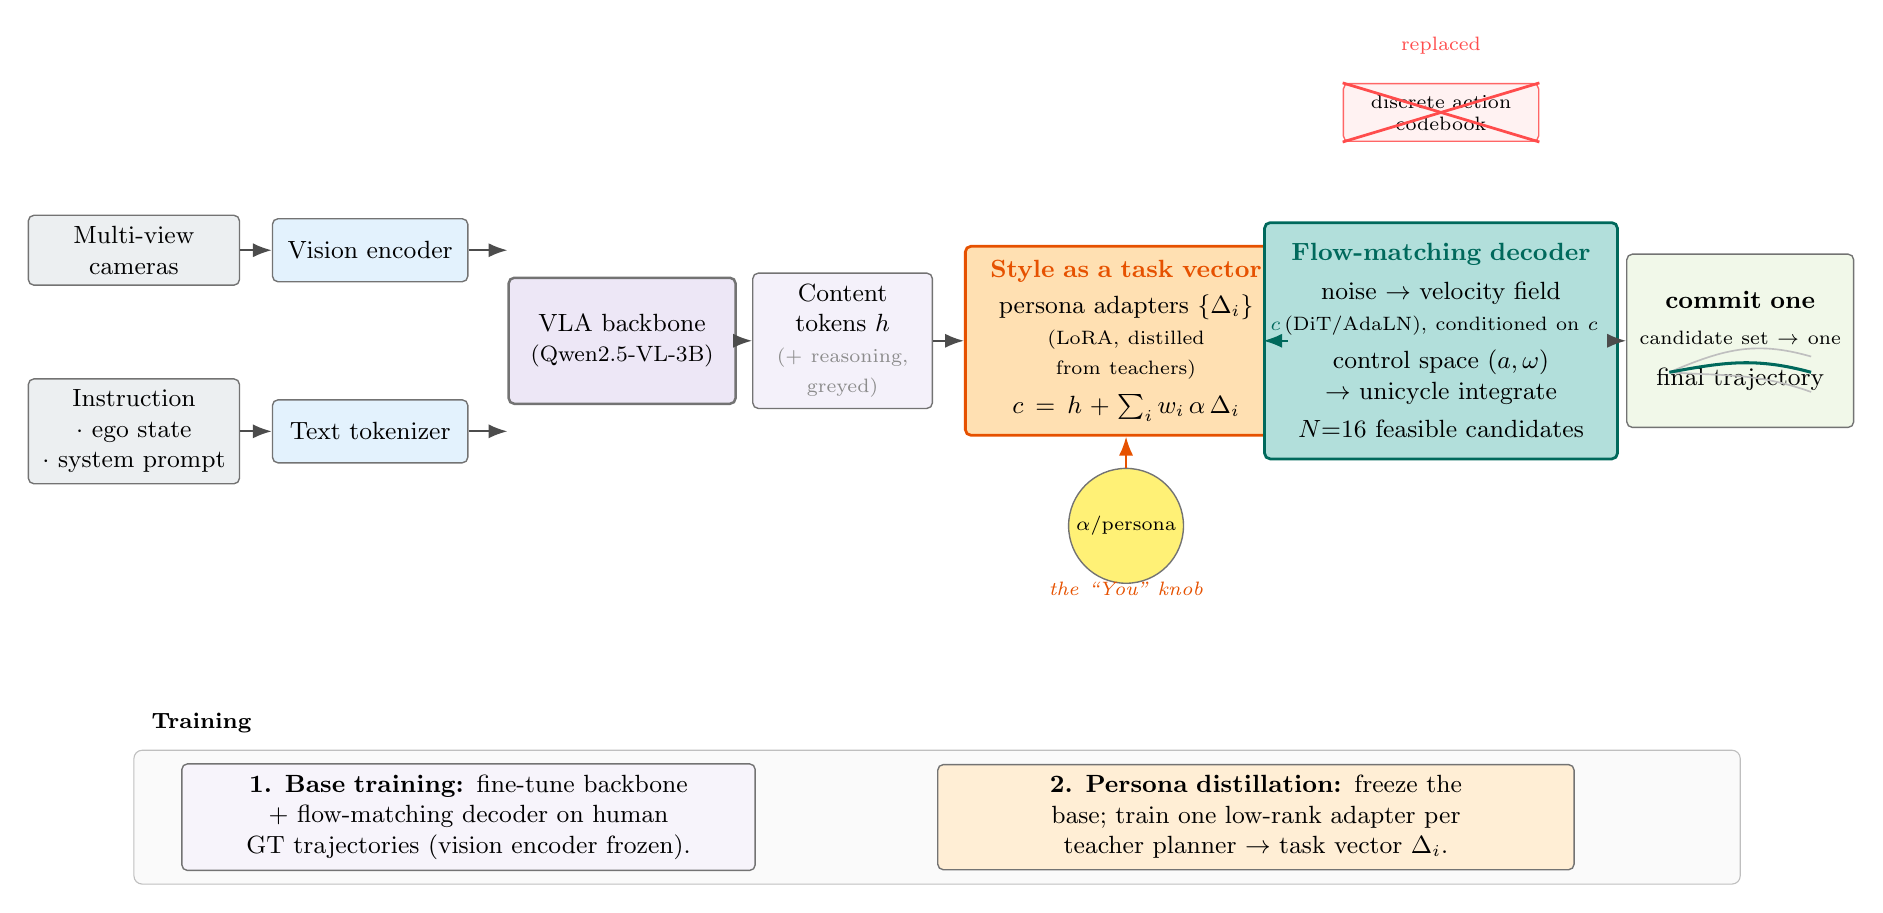
\begin{tikzpicture}[
  font=\small,
  >={Latex[length=2.4mm]},
  box/.style={rounded corners=2pt,draw=black!55,line width=0.5pt,align=center,inner sep=4pt},
  io/.style={box,fill=cIn,text width=24mm},
  enc/.style={box,fill=cEnc,text width=22mm,minimum height=8mm},
  back/.style={box,fill=cBack,line width=0.9pt,text width=26mm,minimum height=16mm},
  tok/.style={box,fill=cBack!60,text width=20mm},
  flow/.style={->,line width=0.7pt,black!70},
]

% ---------- INPUTS ----------
\node[io] (cam) at (0,1.15) {Multi-view\\cameras};
\node[io] (txt) at (0,-1.15) {Instruction $\cdot$ ego state\\$\cdot$ system prompt};

% ---------- ENCODERS ----------
\node[enc] (venc) at (3.0,1.15) {Vision encoder};
\node[enc] (tenc) at (3.0,-1.15) {Text tokenizer};

% ---------- BACKBONE ----------
\node[back] (vla) at (6.2,0) {VLA backbone\\ \footnotesize (Qwen2.5-VL-3B)};

% ---------- CONTENT TOKENS ----------
\node[tok] (h) at (9.0,0) {Content tokens $h$\\ {\scriptsize\color{black!45}(+ reasoning, greyed)}};

% ---------- STYLE TASK-VECTOR BLOCK ----------
\node[box,fill=cStyle,draw=cStyleE,line width=1pt,text width=38mm,minimum height=24mm] (style) at (12.6,0)
  {\textbf{\color{cStyleE}Style as a task vector}\\[2pt]
   persona adapters $\{\Delta_i\}$\\ {\scriptsize (LoRA, distilled from teachers)}\\[3pt]
   $c = h + \sum_i w_i\,\alpha\,\Delta_i$};
\node[box,fill=cKnob,draw=black!55,circle,inner sep=2pt,minimum size=11mm] (knob) at (12.6,-2.35)
  {\scriptsize $\alpha$/persona};
\node[font=\scriptsize\itshape,text=cStyleE] at (12.6,-3.15) {the ``You'' knob};
\draw[flow,cStyleE] (knob) -- (style);

% ---------- FLOW-MATCHING DECODER BLOCK ----------
\node[box,fill=cFM,draw=cFME,line width=1pt,text width=42mm,minimum height=30mm] (fm) at (16.6,0)
  {\textbf{\color{cFME}Flow-matching decoder}\\[3pt]
   noise $\rightarrow$ velocity field\\ {\scriptsize (DiT/AdaLN), conditioned on $c$}\\[3pt]
   control space $(a,\omega)$\\ $\rightarrow$ unicycle integrate\\[3pt]
   $N{=}16$ feasible candidates};

% crossed-out codebook (what FM replaces)
\node[box,fill=red!5,draw=red!60,text width=22mm,font=\scriptsize] (cb) at (16.6,2.9)
  {discrete action codebook};
\draw[red!70,line width=1pt] (cb.south west) -- (cb.north east);
\draw[red!70,line width=1pt] (cb.north west) -- (cb.south east);
\node[font=\scriptsize,text=red!70] at (16.6,3.75) {replaced};

% ---------- COMMIT / OUTPUT ----------
\node[box,fill=cOut,text width=26mm,minimum height=22mm] (out) at (20.4,0)
  {\textbf{commit one}\\[2pt] {\scriptsize candidate set $\rightarrow$ one}\\[4pt]
   final trajectory};
% little trajectory sketch inside out
\begin{scope}[shift={($(out.center)+(0,-0.35)$)}]
  \draw[black!25,line width=0.6pt] (-0.9,-0.05) .. controls (-0.2,0.25) and (0.2,0.35) .. (0.9,0.15);
  \draw[black!25,line width=0.6pt] (-0.9,-0.05) .. controls (-0.2,-0.1) and (0.2,-0.05) .. (0.9,-0.3);
  \draw[cFME,line width=1.1pt] (-0.9,-0.05) .. controls (-0.2,0.08) and (0.2,0.14) .. (0.9,-0.05);
\end{scope}

% ---------- MAIN ARROWS ----------
\draw[flow] (cam) -- (venc);
\draw[flow] (txt) -- (tenc);
\draw[flow] (venc) -- (vla.west|-venc);
\draw[flow] (tenc) -- (vla.west|-tenc);
\draw[flow] (vla) -- (h);
\draw[flow] (h) -- (style);
\draw[flow,cFME] (style) -- (fm) node[midway,above,font=\scriptsize]{$c$};
\draw[flow] (fm) -- (out);

% ---------- TRAINING STRIP ----------
\begin{scope}[on background layer]
  \node[fill=cTrain,rounded corners=3pt,draw=black!25,fit={(0,-5.2)(20.4,-6.9)},inner sep=0pt] (trainbg) {};
\end{scope}
\node[font=\footnotesize\bfseries,anchor=west] at (0.1,-4.85) {Training};
\node[box,fill=cBack!45,text width=70mm,anchor=west] (tr1) at (0.6,-6.05)
  {\textbf{1. Base training:} fine-tune backbone $+$ flow-matching decoder on human GT trajectories (vision encoder frozen).};
\node[box,fill=cStyle!55,text width=78mm,anchor=west] (tr2) at (10.2,-6.05)
  {\textbf{2. Persona distillation:} freeze the base; train one low-rank adapter per teacher planner $\rightarrow$ task vector $\Delta_i$.};

\end{tikzpicture}
\end{document}
